\chapter{O sangue e o sistema circulatório}\label{ch:b2:blood-circulation}

Em 1628, William Harvey fez uma conta. O coração, estimou ele, contém
cerca de duas onças de \omterm{def:b2:blood-circulation:blood}{sangue} e bate setenta vezes por minuto; mesmo
que apenas uma fração disso fosse expelida a cada batimento, o coração
bombearia em uma hora várias vezes o peso do corpo inteiro. O \omterm{def:b2:blood-circulation:blood}{sangue}
não podia ser produzido e consumido nesse ritmo, como Galeno ensinara
durante catorze séculos; ele precisava circular sem parar. Depois ele o
mostrou: amarre um cordão em torno do braço, e as \omterm{def:b2:blood-circulation:vessels}{veias} abaixo do
cordão incham, não as de cima; empurre o \omterm{def:b2:blood-circulation:blood}{sangue} de uma \omterm{def:b2:blood-circulation:vessels}{veia} em direção
à mão, para além de uma válvula, e ele não passa. O \omterm{def:b2:blood-circulation:blood}{sangue} é bombeado
para fora pelas \omterm{def:b2:blood-circulation:vessels}{artérias}, volta pelas \omterm{def:b2:blood-circulation:vessels}{veias}, e os cinco litros inteiros
passam pelo coração a cada minuto. Este capítulo trata desse sistema
fechado --- o que é o \omterm{def:b2:blood-circulation:blood}{sangue}, como ele é encaminhado, a física de seu
escoamento pelos vasos, da aorta a um \omterm{def:b2:blood-circulation:vessels}{capilar}, e as trocas nos
\omterm{def:b2:blood-circulation:vessels}{capilares}, que são a razão de ser de tudo isso.

\section{O sangue}

\begin{definition}[A composição do sangue]\label{def:b2:blood-circulation:blood}
\index{sangue}\index{plasma}\index{hematócrito}\index{hemácia}\index{plaqueta}
O sangue é um tecido em suspensão: cerca de \qty{5}{L} num adulto,
\qty{7}{\%} da massa corporal. Centrifugado, ele se separa em
\emph{plasma} (\qty{55}{\%}: água, \qty{70}{g/L} de proteínas ---
albumina, globulinas, fibrinogênio --- e os sais, açúcares, lipídios,
gases e hormônios que ele transporta) e células (\qty{45}{\%}, o
\emph{hematócrito}): as \emph{hemácias} ($5\times 10^{12}$ por litro,
discos bicôncavos de \qty{7}{\micro m} sem núcleo, cada um repleto de
\num{280} milhões de moléculas de hemoglobina, que vivem 120 dias e são
produzidos na medula óssea à razão de dois milhões por segundo), os
\emph{leucócitos} ($7\times 10^{9}$ por litro: neutrófilos, linfócitos,
monócitos, eosinófilos, basófilos, o braço móvel da imunidade) e as
\emph{plaquetas} ($3\times 10^{11}$ por litro, fragmentos de células da
medula que tampam feridas e iniciam a coagulação). As hemácias
transportam o oxigênio --- \qty{200}{mL} por litro de sangue em
saturação total, setenta vezes o que a água dissolve --- e o plasma
transporta todo o resto, inclusive os \qty{20}{\%} do $\mathrm{CO_2}$
que não estão nas células, o calor dos músculos até a pele e os
hormônios do \cref{ch:b2:cell-signalling} até seus alvos. O sangue é também uma solução
sob \emph{\omterm{thm:b2:blood-circulation:oncotic}{pressão oncótica}}: suas proteínas, que não conseguem sair dos
\omterm{def:b2:blood-circulation:vessels}{capilares}, exercem uma atração osmótica de cerca de \qty{25}{mmHg}, e é
essa atração que mantém o plasma nos vasos.
\end{definition}

\begin{omfigure}
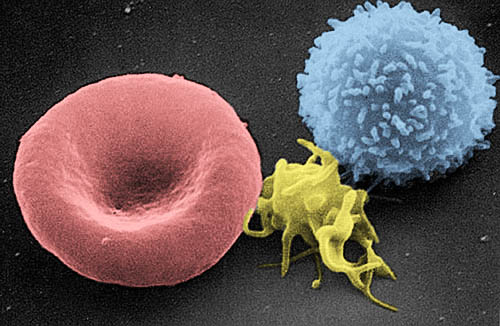
\includegraphics[width=0.5\linewidth]{images/book3/red-cells-nci.jpg}

{\small Uma \omterm{def:b2:blood-circulation:blood}{hemácia}, uma \omterm{def:b2:blood-circulation:blood}{plaqueta} e um leucócito (um linfócito) ao
microscópio eletrônico de varredura: os três componentes celulares do
\omterm{def:b2:blood-circulation:blood}{sangue}, na mesma escala.}
\end{omfigure}

\begin{proposition}[A hemostasia]\label{prop:b2:blood-circulation:clotting}
\index{hemostasia}\index{cascata da coagulação}\index{fibrina}
Um vaso cortado é vedado em três etapas, em poucos minutos. O vaso se
contrai; as \omterm{def:b2:blood-circulation:blood}{plaquetas} aderem ao colágeno exposto, liberam sinais que
recrutam e ativam mais \omterm{def:b2:blood-circulation:blood}{plaquetas} e formam um tampão; e uma
\emph{cascata} de proteases plasmáticas, cada uma ativando a seguinte
(uma dúzia de fatores de coagulação, a maioria produzida no fígado,
vários dependentes da vitamina K), converte o fibrinogênio em
\emph{fibrina} insolúvel, cujos fios entrelaçam o tampão num coágulo.
Uma cascata amplifica: um traço do desencadeador (o fator tecidual da
parede lesada) termina em gramas de fibrina. Ela também precisa ser
contida: anticoagulantes do \omterm{def:b2:blood-circulation:blood}{plasma} (antitrombina, proteína C) e do
endotélio intacto confinam o coágulo à ferida, e um segundo sistema, a
fibrinólise, o dissolve à medida que o vaso cicatriza. A hemofilia é a
falta de um fator; uma trombose é um coágulo onde nenhum era desejado,
e a principal causa de morte nos países ricos é um coágulo numa
\omterm{def:b2:blood-circulation:vessels}{artéria} coronária ou cerebral.
\end{proposition}

\section{Os circuitos}

\begin{definition}[Aberta e fechada, simples e dupla]\label{def:b2:blood-circulation:circuits}
\index{circulação aberta}\index{circulação fechada}\index{circulação dupla}\index{circulação pulmonar}\index{circulação sistêmica}
Numa circulação \emph{aberta} (insetos, a maioria dos moluscos), um
coração bombeia o \omterm{def:b2:blood-circulation:blood}{sangue} para uma cavidade do corpo, onde ele banha
diretamente os órgãos e volta a baixa pressão; o fluxo é lento e mal
direcionado, e os insetos separaram o problema dos gases do \omterm{def:b2:blood-circulation:blood}{sangue}
levando o ar por tubos diretamente aos tecidos. Numa circulação
\emph{fechada} (anelídeos, cefalópodes, vertebrados), o \omterm{def:b2:blood-circulation:blood}{sangue}
permanece nos vasos e é impulsionado através dos \omterm{def:b2:blood-circulation:vessels}{capilares} sob
pressão, de modo que sua distribuição pode ser controlada órgão por
órgão. Os peixes têm um circuito \emph{simples}: coração $\to$
brânquias $\to$ corpo $\to$ coração, de modo que o \omterm{def:b2:blood-circulation:blood}{sangue} chega aos
tecidos com a baixa pressão que resta após os \omterm{def:b2:blood-circulation:vessels}{capilares} das brânquias.
Os mamíferos e as aves têm um circuito \emph{duplo}: o coração direito
impulsiona a circulação \emph{pulmonar} (pulmões, baixa pressão,
\qty{25}{mmHg} de sistólica) e o coração esquerdo, depois que o \omterm{def:b2:blood-circulation:blood}{sangue}
volta, impulsiona a circulação \emph{sistêmica} (corpo, alta pressão,
\qty{120}{mmHg}); as duas bombas estão em série e movem o mesmo fluxo,
cerca de \qty{5}{L} por minuto em repouso. Os anfíbios e a maioria dos
répteis têm um coração com um único ventrículo, que mistura
parcialmente as duas correntes --- o estágio intermediário. O circuito
duplo é o que torna possível um metabolismo de sangue quente: alta
pressão para todos os órgãos e um pulmão protegido dela.
\end{definition}
\begin{proof}[Evidências]
Harvey (1628) argumentou pela quantidade --- o débito calculado acima ---
e pela estrutura: as válvulas das \omterm{def:b2:blood-circulation:vessels}{veias}, que Fabricius descrevera, só
permitem o fluxo em direção ao coração, como ele mostrou pressionando
as \omterm{def:b2:blood-circulation:vessels}{veias} de um braço garroteado; as válvulas do coração só permitem o
fluxo dos átrios para os ventrículos e para as \omterm{def:b2:blood-circulation:vessels}{artérias}; e o \omterm{def:b2:blood-circulation:blood}{sangue}
jorra das \omterm{def:b2:blood-circulation:vessels}{artérias} e escorre das \omterm{def:b2:blood-circulation:vessels}{veias}. Ele não podia ver os \omterm{def:b2:blood-circulation:vessels}{capilares}
e deduziu sua existência; Malpighi os viu num pulmão de rã em 1661,
quatro anos depois da morte de Harvey.
\end{proof}

\begin{omfigure}
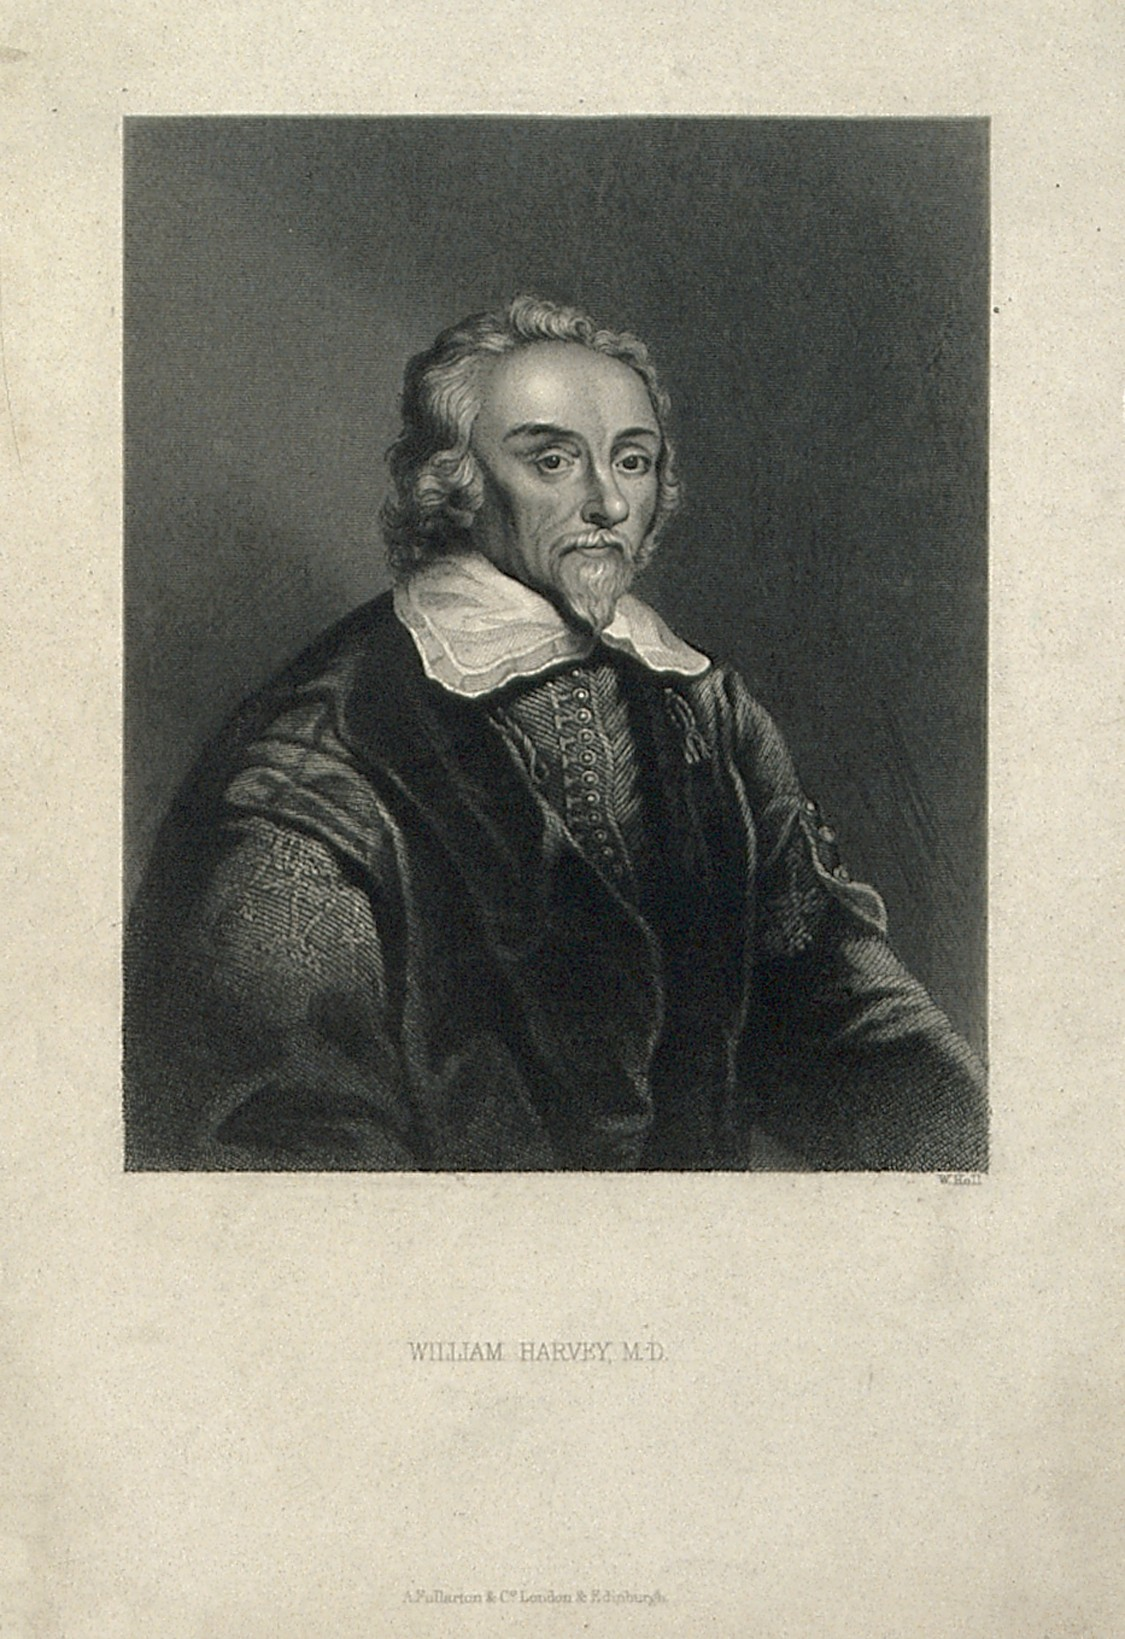
\includegraphics[width=0.3\linewidth]{images/book4/harvey.jpg}\hspace{0.05\linewidth}
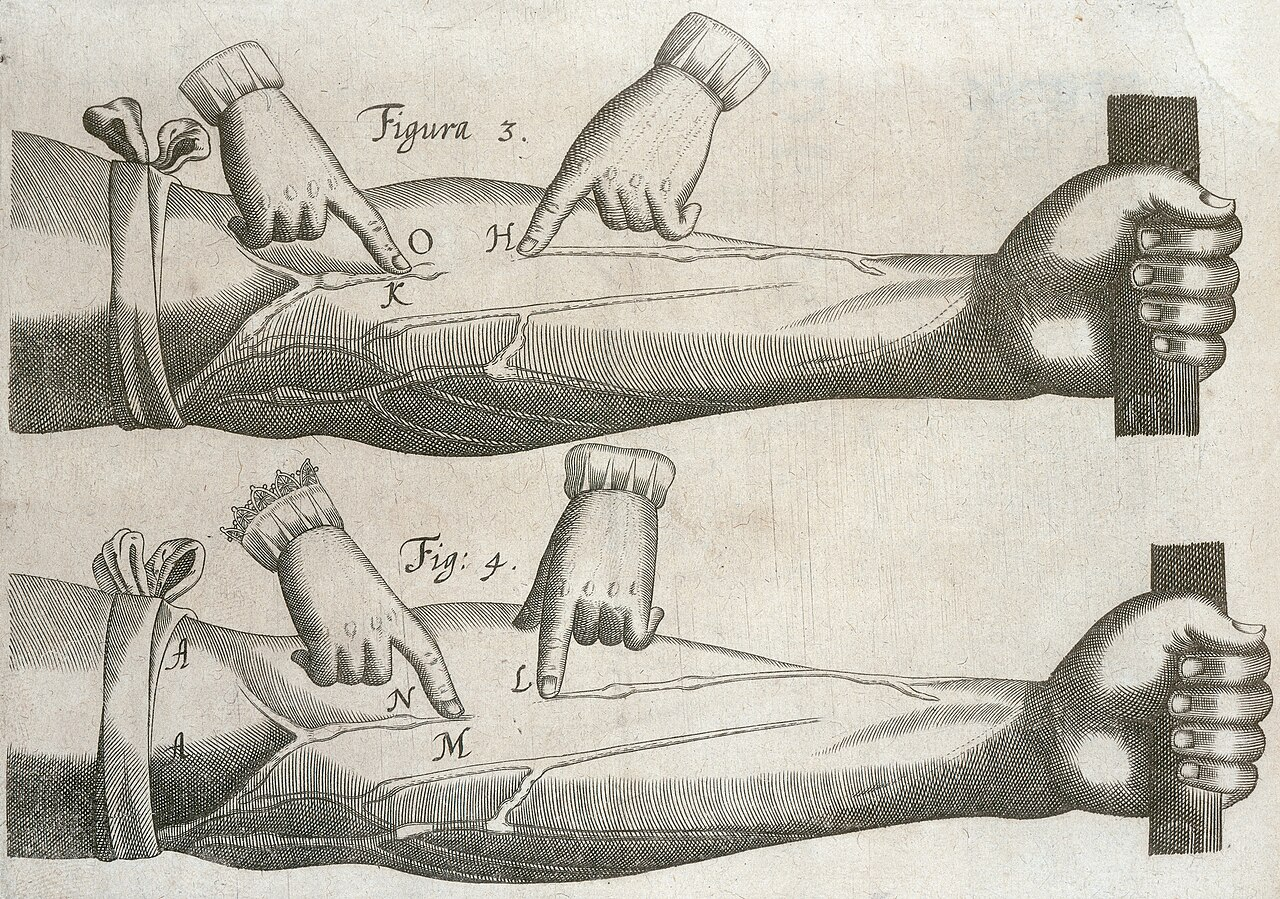
\includegraphics[width=0.42\linewidth]{images/book4/harvey-veins.jpg}

{\small William Harvey e a prancha de seu livro de 1628: as \omterm{def:b2:blood-circulation:vessels}{veias} de um
antebraço garroteado incham abaixo do cordão, e o \omterm{def:b2:blood-circulation:blood}{sangue} empurrado em
direção à mão para nas válvulas.}
\end{omfigure}

\begin{omfigure}
\begin{tikzpicture}[every node/.style={font=\scriptsize}, >=stealth]
  % lungs and body
  \node[draw, rounded corners, fill=omDef!12, minimum width=3.4cm, minimum height=0.9cm] (lung) at (0,3) {pulmões: capilares pulmonares};
  \node[draw, rounded corners, fill=omExo!25, minimum width=3.4cm, minimum height=0.9cm] (body) at (0,-3) {corpo: capilares sistêmicos};
  % heart chambers
  \node[draw, fill=omDef!25, minimum width=1.3cm, minimum height=0.7cm] (ra) at (-1.6,0.6) {átrio direito};
  \node[draw, fill=omDef!35, minimum width=1.3cm, minimum height=0.9cm] (rv) at (-1.6,-0.5) {ventrículo direito};
  \node[draw, fill=omThm!20, minimum width=1.3cm, minimum height=0.7cm] (la) at (1.6,0.6) {átrio esquerdo};
  \node[draw, fill=omThm!35, minimum width=1.3cm, minimum height=0.9cm] (lv) at (1.6,-0.5) {ventrículo esquerdo};
  \draw[->, thick] (ra) -- (rv); \draw[->, thick] (la) -- (lv);
  % pulmonary circuit
  \draw[->, very thick, omDef] (rv.west) -- ++(-1.4,0) |- (lung.west) node[pos=0.25, left, align=right] {artéria pulmonar\\\qty{25}{mmHg}};
  \draw[->, very thick, omThm] (lung.east) -| (la.east) node[pos=0.75, right, align=left] {veias pulmonares\\oxigenadas};
  % systemic circuit
  \draw[->, very thick, omThm] (lv.east) -- ++(1.4,0) |- (body.east) node[pos=0.25, right, align=left] {aorta\\\qty{120}{mmHg}};
  \draw[->, very thick, omDef] (body.west) -| (ra.west);
  \node[omDef, anchor=east, align=right] at (-2.45,-1.6) {veias cavas\\\qty{5}{mmHg}};
  \node[anchor=north, align=center] at (0,-3.7) {o mesmo fluxo nos dois circuitos:\\\qty{5}{L/min} em repouso};
\end{tikzpicture}

{\small A \omterm{def:b2:blood-circulation:circuits}{circulação dupla}. O coração direito envia o \omterm{def:b2:blood-circulation:blood}{sangue} através dos
pulmões a baixa pressão; o coração esquerdo o envia pelo corpo a alta
pressão; as duas bombas, em série, movem o mesmo volume por minuto.}
\end{omfigure}

\section{Os vasos e a física do escoamento}

\begin{definition}[A árvore vascular]\label{def:b2:blood-circulation:vessels}
\index{artéria}\index{arteríola}\index{capilar}\index{veia}
O \omterm{def:b2:blood-circulation:blood}{sangue} sai do coração pelas \emph{artérias}: tubos de parede espessa,
com camadas elásticas que se esticam a cada batimento e se retraem
entre os batimentos, suavizando os pulsos num fluxo mais constante (a
aorta tem \qty{2.5}{cm} de diâmetro). Elas se ramificam em
\emph{arteríolas}, vasos de um décimo de milímetro ou menos cujas
paredes são sobretudo músculo liso: contraindo-se ou relaxando, uma
arteríola muda seu raio e, portanto, de modo acentuado, sua resistência
--- as arteríolas são as torneiras da circulação e o local da maior
parte da queda de pressão. Elas se abrem em \emph{capilares}: tubos
formados por uma única célula endotelial enrolada em torno de uma luz
de \qtyrange{5}{10}{\micro m}, com cerca de \qty{1}{mm} de comprimento,
uns quarenta bilhões deles, com uma superfície total próxima de
\qty{600}{m^2}, através de cujas paredes ocorrem todas as trocas. Os
capilares drenam para vênulas e \emph{veias}: de parede fina,
distensíveis, contendo dois terços do \omterm{def:b2:blood-circulation:blood}{sangue} a baixa pressão, com
válvulas que mantêm o fluxo em direção ao coração enquanto os músculos
as comprimem. Todo vaso é revestido por uma única camada de
\emph{endotélio}, que não é um revestimento passivo, mas uma glândula
--- libera óxido nítrico para relaxar a arteríola e sinais que recrutam
leucócitos --- e um filtro.
\end{definition}

\begin{omfigure}
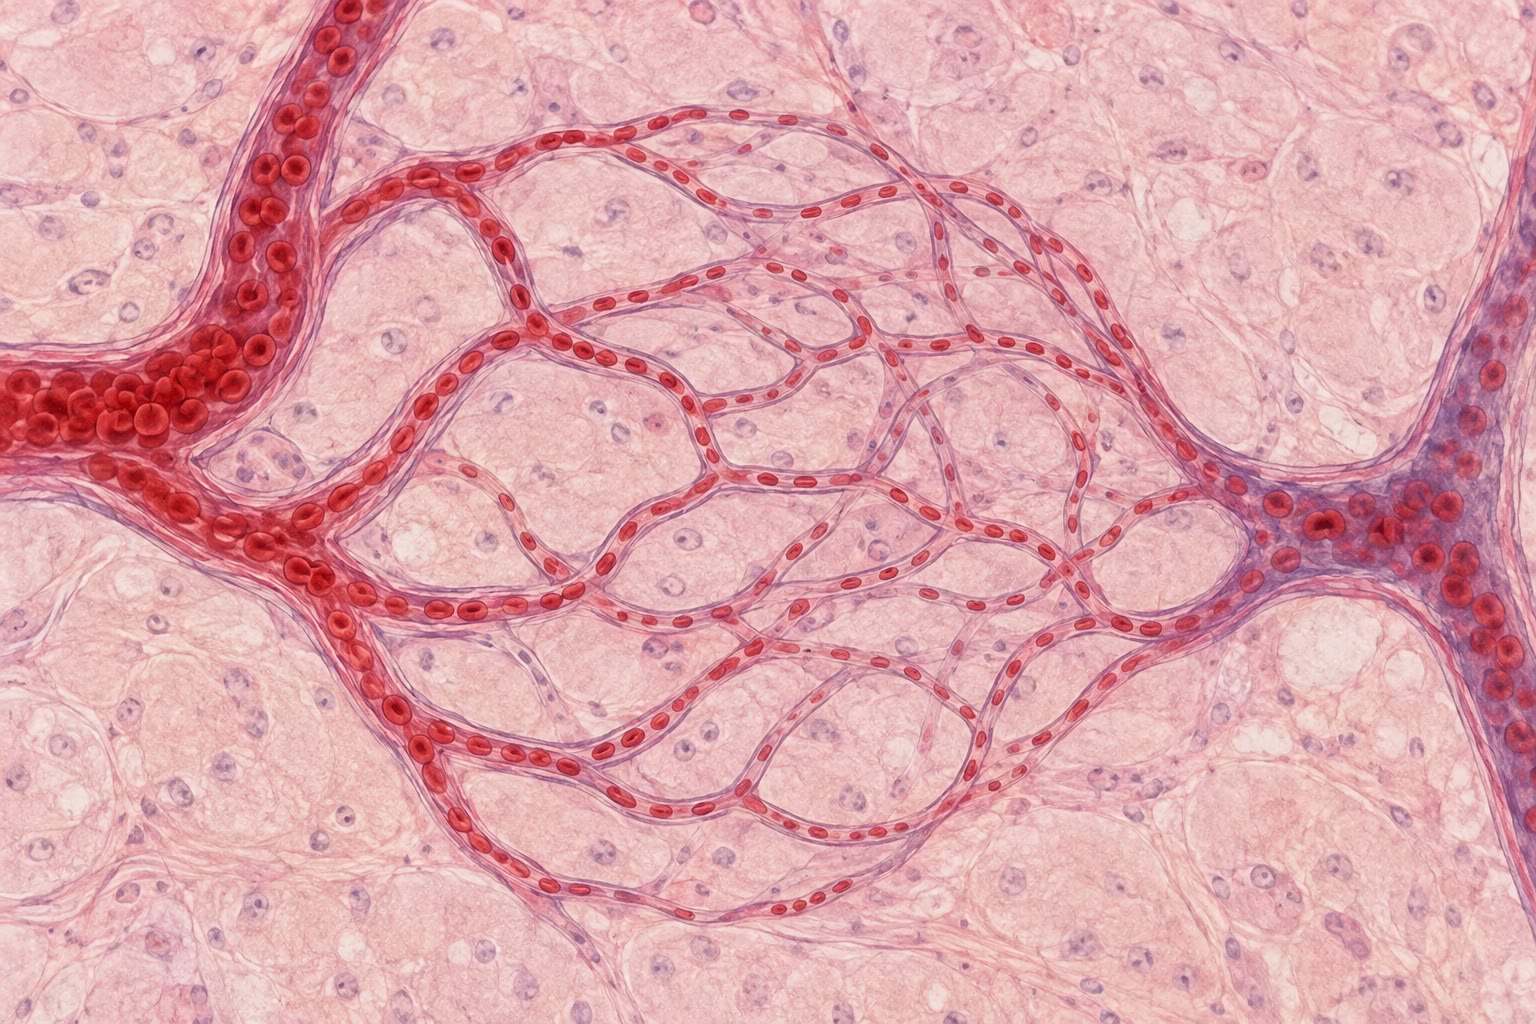
\includegraphics[width=0.55\linewidth]{images/book4/ai/b4-16-capillary-bed.jpg}

{\small Um leito \omterm{def:b2:blood-circulation:vessels}{capilar}: uma \omterm{def:b2:blood-circulation:vessels}{arteríola} que alimenta uma rede de
\omterm{def:b2:blood-circulation:vessels}{capilares} nos quais as \omterm{def:b2:blood-circulation:blood}{hemácias} passam em fila única e que voltam a se
reunir numa vênula.}
\end{omfigure}

\begin{theorem}[A lei de Poiseuille e a resistência vascular]\label{thm:b2:blood-circulation:poiseuille}
\index{lei de Poiseuille}\index{resistência vascular}
O fluxo estacionário $Q$ de um fluido de viscosidade $\eta$ através de
um tubo de raio $r$ e comprimento $L$ sob uma diferença de pressão
$\Delta P$ é
\[
Q = \frac{\pi r^{4}}{8\eta L}\,\Delta P, \qquad \text{de modo que}\qquad
R \equiv \frac{\Delta P}{Q} = \frac{8\eta L}{\pi r^{4}} .
\]
A resistência diminui com a \emph{quarta potência} do raio: uma
\omterm{def:b2:blood-circulation:vessels}{arteríola} que reduz seu raio em \qty{20}{\%} multiplica sua resistência
por $1/0.8^{4} = 2.4$, e uma que o reduz à metade, por 16. É por isso
que alguns milímetros de músculo arteriolar conseguem redirecionar o
\omterm{def:b2:blood-circulation:blood}{sangue} do corpo inteiro --- para o intestino após uma refeição, para os
músculos no exercício, para a pele no calor --- e por isso que a pressão
cai de \qty{95}{mmHg} nas pequenas \omterm{def:b2:blood-circulation:vessels}{artérias} para \qty{35}{mmHg} na
entrada dos \omterm{def:b2:blood-circulation:vessels}{capilares}, quase toda ela através das \omterm{def:b2:blood-circulation:vessels}{arteríolas}, enquanto
a queda ao longo da aorta é uma fração de milímetro de mercúrio.
\end{theorem}
\begin{proof}
No escoamento laminar estacionário, o fluido se move em camadas
concêntricas; a força viscosa entre as camadas equilibra a pressão.
Para o cilindro de raio $s < r$, a força de pressão $\pi s^{2}\Delta P$
é igual ao arrasto viscoso sobre sua superfície,
$2\pi s L\,\eta\,(-\mathrm{d}v/
\mathrm{d}s)$, de modo que $\mathrm{d}v/\mathrm{d}s = -s\Delta P/(2\eta L)$
e, com $v(r) = 0$, $v(s) = (\Delta P/4\eta L)(r^{2} - s^{2})$ --- um
perfil parabólico. Integrando a velocidade sobre a seção transversal,
$Q = \int_{0}^{r} v\,2\pi s\,\mathrm{d}s = (\pi\Delta P/2\eta L)
\int_{0}^{r}(r^{2}s - s^{3})\,\mathrm{d}s = \pi r^{4}\Delta P/8\eta
L$. (O \omterm{def:b2:blood-circulation:blood}{sangue} não é bem um fluido simples e as \omterm{def:b2:blood-circulation:vessels}{artérias} não são
rígidas, mas a lei da quarta potência vale bem o bastante para fazer um
corpo funcionar.)
\end{proof}

\begin{theorem}[Continuidade: onde o sangue desacelera]\label{thm:b2:blood-circulation:continuity}
\index{equação da continuidade}
O mesmo volume por segundo passa por todos os níveis da árvore, de modo
que a velocidade média num nível é $v = Q/A$, em que $A$ é a área de
seção transversal \emph{total} de todos os vasos desse nível. A aorta
(\qty{3}{cm^2}) leva \qty{5}{L/min} a \qty{28}{cm/s}; os \omterm{def:b2:blood-circulation:vessels}{capilares},
com uma seção transversal total perto de \qty{3000}{cm^2}, o levam a
\qty{0.03}{cm/s}, de modo que uma \omterm{def:b2:blood-circulation:blood}{hemácia} leva cerca de três segundos para
atravessar um \omterm{def:b2:blood-circulation:vessels}{capilar} --- tempo suficiente para que seu oxigênio se
difunda para fora (\cref{ch:b2:unicellular-diversity}: um micrômetro em um milissegundo). As
\omterm{def:b2:blood-circulation:vessels}{veias}, com seção total menor que a dos \omterm{def:b2:blood-circulation:vessels}{capilares}, voltam a acelerar o
\omterm{def:b2:blood-circulation:blood}{sangue} até \qty{10}{cm/s} nas \omterm{def:b2:blood-circulation:vessels}{veias} cavas. A árvore é construída de
modo que o \omterm{def:b2:blood-circulation:blood}{sangue} seja lento exatamente onde precisa fazer trocas e
rápido em todo o resto.
\end{theorem}
\begin{proof}
Conservação do volume: o que entra num nível por segundo sai dele, de
modo que $Q = A\,v$ é o mesmo em todos os níveis. $\qty{5}{L/min} =
\qty{83}{cm^3/s}$; $83/3 = \qty{28}{cm/s}$; $83/3000 =
\qty{0.028}{cm/s}$.
\end{proof}

\begin{omfigure}
\begin{tikzpicture}
\begin{axis}[
  width=0.9\linewidth, height=6.4cm,
  axis x line=bottom, axis y line=left,
  xmin=0, xmax=7, ymin=0, ymax=130,
  xtick={0.5,1.5,2.5,3.5,4.5,5.5,6.5},
  xticklabels={aorta, artérias, arteríolas, capilares, vênulas, veias, veias cavas},
  x tick label style={font=\scriptsize, rotate=30, anchor=north east},
  ylabel={pressão (\unit{mmHg})}, ylabel style={font=\small, omThm},
  tick label style={font=\small}, ytick={0,40,80,120},
  legend style={font=\scriptsize, at={(0.97,0.95)}, anchor=north east, draw=none},
  clip=false,
]
\addplot[very thick, omThm] coordinates {(0,120) (0.5,118) (1,110) (1.5,100) (2,95) (2.5,60) (3,35) (3.5,25) (4,15) (4.5,12) (5,8) (5.5,5) (6,4) (6.5,3) (7,2)};
\addlegendentry{pressão média}
\addplot[very thick, omThm, dashed] coordinates {(0,120) (0.5,120) (1,125) (1.5,120) (2,100)};
\addplot[very thick, omThm, dashed] coordinates {(0,80) (0.5,80) (1,80) (1.5,82) (2,88)};
\addlegendentry{sistólica e diastólica}
\end{axis}
\begin{axis}[
  width=0.9\linewidth, height=6.4cm,
  axis x line=none, axis y line=right,
  xmin=0, xmax=7, ymin=0, ymax=32,
  ylabel={velocidade (\unit{cm/s})}, ylabel style={font=\small, omDef},
  tick label style={font=\small}, ytick={0,10,20,30},
  legend style={font=\scriptsize, at={(0.97,0.72)}, anchor=north east, draw=none},
  clip=false,
]
\addplot[very thick, omDef] coordinates {(0,28) (0.5,26) (1,18) (1.5,10) (2,5) (2.5,1.5) (3,0.3) (3.5,0.03) (4,0.3) (4.5,1.5) (5,4) (5.5,7) (6,9) (6.5,10) (7,10)};
\addlegendentry{velocidade média}
\end{axis}
\end{tikzpicture}

{\small A pressão (vermelho) e a velocidade média (azul) ao longo da
\omterm{def:b2:blood-circulation:circuits}{circulação sistêmica}. O pulso é suavizado nas \omterm{def:b2:blood-circulation:vessels}{artérias}, a pressão cai
sobretudo através das \omterm{def:b2:blood-circulation:vessels}{arteríolas}, e o \omterm{def:b2:blood-circulation:blood}{sangue} é mais lento nos
\omterm{def:b2:blood-circulation:vessels}{capilares}, onde a seção transversal total é mil vezes a da aorta.}
\end{omfigure}

\begin{theorem}[A artéria elástica como reservatório]\label{thm:b2:blood-circulation:windkessel}
\index{Windkessel}\index{complacência!arterial}\index{pressão de pulso}
O coração ejeta em jatos; os tecidos recebem um fluxo quase constante.
As grandes \omterm{def:b2:blood-circulation:vessels}{artérias} fazem a suavização: esticam-se durante a ejeção,
armazenando parte do volume sistólico, e se retraem durante a diástole,
impulsionando-o adiante. Se as \omterm{def:b2:blood-circulation:vessels}{artérias} têm uma \emph{complacência}
$C$ (volume armazenado por unidade de pressão) e as \omterm{def:b2:blood-circulation:vessels}{arteríolas} uma
resistência $R$, então, durante a diástole, com a valva aórtica
fechada, a pressão decai como
\[
P(t) = P_{s}\,e^{-t/RC},
\]
de modo que a pressão diastólica após uma diástole de duração $t_d$ é
$P_s e^{-t_d/RC}$: com $R = \qty{1}{mmHg.s/mL}$, $C =
\qty{2}{mL/mmHg}$ e $t_d = \qty{0.8}{s}$, uma sistólica de
\qty{120}{mmHg} cai para \qty{80}{mmHg}. Uma aorta mais rígida ($C$
menor, como na velhice) deixa a pressão cair mais entre os batimentos e
subir mais durante a ejeção: a \emph{\omterm{thm:b2:blood-circulation:windkessel}{pressão de pulso}} se alarga, e o
coração trabalha contra um pico mais alto.
\end{theorem}
\begin{proof}
Durante a diástole, nenhum \omterm{def:b2:blood-circulation:blood}{sangue} entra nas \omterm{def:b2:blood-circulation:vessels}{artérias}, e o \omterm{def:b2:blood-circulation:blood}{sangue} sai
delas pelas \omterm{def:b2:blood-circulation:vessels}{arteríolas} a $Q = P/R$; o volume arterial diminui a
$\mathrm{d}V/\mathrm{d}t = -P/R$ e, como $\mathrm{d}V = C\,
\mathrm{d}P$, $C\,\mathrm{d}P/\mathrm{d}t = -P/R$, cuja solução é a
exponencial de constante de tempo $RC$. Com $RC = \qty{2}{s}$:
$120\,e^{-0.4} = \qty{80}{mmHg}$.
\end{proof}

\section{As trocas nos capilares}

\begin{proposition}[Dois tipos de troca]\label{prop:b2:blood-circulation:exchange}
\index{trocas capilares}\index{forças de Starling}\index{edema}\index{linfa}
Através da parede \omterm{def:b2:blood-circulation:vessels}{capilar}, os solutos se movem por \emph{difusão} ---
os gases e os lipídios através das células, a água e os pequenos
solutos pelas fendas entre elas, sobre a área enorme e a distância curta
que tornam o fluxo abundante (lei de Fick, como para a \omterm{def:b2:mammal-reproduction:placenta}{placenta} do
\cref{ch:b2:mammal-reproduction}) ---, e a água se move por \emph{fluxo de massa}, impulsionada
pelo equilíbrio entre duas pressões. A pressão hidrostática no
\omterm{def:b2:blood-circulation:vessels}{capilar}, $P_c$, empurra o líquido para fora; a \omterm{thm:b2:blood-circulation:oncotic}{pressão oncótica} das
proteínas plasmáticas, $\pi_c$, o puxa para dentro (\emph{\omterm{prop:b2:blood-circulation:exchange}{forças de
Starling}}). Na extremidade arterial, $P_c \approx
\qty{35}{mmHg}$ supera $\pi_c \approx \qty{25}{mmHg}$ e o líquido é
filtrado para fora; na extremidade venosa, $P_c \approx \qty{15}{mmHg}$
e o líquido é reabsorvido; no corpo inteiro, cerca de \qty{20}{L} por
dia são filtrados e \qty{17}{L} voltam, e o saldo de \qty{3}{L}, com as
proteínas que escaparam, é recolhido pelos vasos \emph{linfáticos} e
devolvido às \omterm{def:b2:blood-circulation:vessels}{veias} no pescoço. O \emph{edema} --- o inchaço por líquido
nos tecidos --- surge sempre que o equilíbrio se rompe: pressão venosa
alta (insuficiência cardíaca), proteínas plasmáticas baixas (desnutrição,
doença hepática ou renal), \omterm{def:b2:blood-circulation:vessels}{capilares} permeáveis (inflamação) ou
linfáticos obstruídos.
\end{proposition}

\begin{omfigure}
\begin{tikzpicture}[every node/.style={font=\scriptsize}, >=stealth]
  % capillary
  \draw[thick, fill=omThm!10] (0,0) rectangle (9,1.2);
  \node[left] at (-0.1,0.6) {arteríola};
  \node[right] at (9.1,0.6) {vênula};
  \draw[->, very thick, omThm] (0.3,0.6) -- (8.7,0.6);
  % pressures
  \node[above, align=center] at (1.5,1.3) {extremidade arterial\\$P_c = 35$, $\pi_c = 25$};
  \node[above, align=center] at (7.5,1.3) {extremidade venosa\\$P_c = 15$, $\pi_c = 25$};
  \foreach \x in {0.8,1.5,2.2} \draw[->, thick, omDef] (\x,0) -- (\x,-0.7);
  \node[below, align=center, omDef] at (1.5,-0.75) {saldo $+10$ mmHg:\\filtração};
  \foreach \x in {6.8,7.5,8.2} \draw[->, thick, omDef] (\x,-0.7) -- (\x,0);
  \node[below, align=center, omDef] at (7.5,-0.75) {saldo $-10$ mmHg:\\reabsorção};
  \draw[->, thick, omExo!70!black] (4.5,-0.4) -- (4.5,-1.6) node[below, align=center] {excesso para a linfa:\\\qty{3}{L} por dia};
  \node[align=center] at (4.5,-0.15) {líquido intersticial};
\end{tikzpicture}

{\small As \omterm{prop:b2:blood-circulation:exchange}{forças de Starling} ao longo de um \omterm{def:b2:blood-circulation:vessels}{capilar}. A pressão
hidrostática empurra o líquido para fora e a \omterm{thm:b2:blood-circulation:oncotic}{pressão oncótica} das
proteínas plasmáticas o puxa de volta; a filtração na extremidade
arterial supera a reabsorção na extremidade venosa, e a linfa devolve a
diferença.}
\end{omfigure}

\begin{theorem}[A pressão oncótica]\label{thm:b2:blood-circulation:oncotic}
\index{pressão oncótica}\index{albumina}
Uma solução de $c$ mols por litro de um soluto que não consegue
atravessar uma membrana exerce através dela uma pressão osmótica
$\pi = cRT$ (van 't Hoff). A albumina plasmática, \qty{40}{g/L} de uma
proteína de massa molar \qty{66}{kg/mol}, corresponde a
$c = \qty{0.6}{mmol/L}$ e dá $\pi =
0.6\times 8.314\times 310 = \qty{1.55}{kPa} \approx \qty{12}{mmHg}$;
as outras proteínas e os íons adicionais que a carga negativa da
albumina retém elevam o total para cerca de \qty{25}{mmHg}. O cloreto
de sódio do \omterm{def:b2:blood-circulation:blood}{plasma}, a \qty{150}{mmol/L}, exerceria \qty{5800}{mmHg}
--- mas ele atravessa livremente a parede \omterm{def:b2:blood-circulation:vessels}{capilar} e não exerce nenhuma
pressão através dela. O que importa para o \omterm{def:b2:blood-circulation:vessels}{capilar} é a proteína: reduza
a albumina à metade, como numa doença renal que a perde na urina, e a
atração que reabsorve cai à metade, o líquido se acumula nos tecidos e
o paciente incha.
\end{theorem}
\begin{proof}
$\qty{40}{g/L}/\qty{66000}{g/mol} = \qty{6.1e-4}{mol/L} =
\qty{0.61}{mol/m^3}$; $\pi = cRT = 0.61\times 8.314\times 310 =
\qty{1570}{Pa}$; $\qty{1}{mmHg} = \qty{133}{Pa}$, logo
\qty{11.8}{mmHg}. A própria lei de van 't Hoff é o limite das soluções
diluídas deduzido no volume do Ano 1.
\end{proof}

\begin{example}[A circulação como sistema de transporte]\label{ex:b2:blood-circulation:transport}
Cinco litros por minuto através de \qty{600}{m^2} de parede \omterm{def:b2:blood-circulation:vessels}{capilar} são
um serviço de entrega sem igual. Ele leva a cada célula oxigênio a
poucos diâmetros celulares de distância (nenhuma célula do corpo fica a
mais de \qty{20}{\micro m} de um \omterm{def:b2:blood-circulation:vessels}{capilar}), remove seu $\mathrm{CO_2}$,
o lactato e a ureia, leva a glicose do fígado ao encéfalo e os ácidos
graxos das reservas de gordura aos músculos, distribui os hormônios do
\cref{ch:b2:cell-signalling} de uma glândula a todos os receptores do corpo em um minuto,
leva o calor do núcleo do corpo à pele e de volta, e transporta os
leucócitos até uma ferida em poucas horas. É também sua
vulnerabilidade: um coágulo, uma hemorragia ou uma bomba que falha
interrompem tudo de uma vez, e o encéfalo, que não armazena combustível,
falha em segundos. O restante desta parte do livro trata da bomba
(\cref{ch:b2:heart}) e de como a pressão é regulada para que o serviço continue
ao ficarmos de pé, ao corrermos e ao sangrarmos (\cref{ch:b2:blood-pressure}).
\end{example}

\section{Exercícios}

\begin{exercise}[$\star$]\label{exo:b2:blood-circulation:1}
Dê a composição do \omterm{def:b2:blood-circulation:blood}{sangue} em volume e o número, o tamanho e a função de
cada componente celular.
\end{exercise}

\begin{exercise}[$\star$]\label{exo:b2:blood-circulation:2}
Desenhe o circuito de um peixe e o de um mamífero, marque as pressões e
diga o que o circuito duplo ganha.
\end{exercise}

\begin{exercise}[$\star$]\label{exo:b2:blood-circulation:3}
Para cada tipo de vaso --- \omterm{def:b2:blood-circulation:vessels}{artéria}, \omterm{def:b2:blood-circulation:vessels}{arteríola}, \omterm{def:b2:blood-circulation:vessels}{capilar}, \omterm{def:b2:blood-circulation:vessels}{veia} --- dê a
estrutura da parede e a função a que ela serve.
\end{exercise}

\begin{exercise}[$\star$]\label{exo:b2:blood-circulation:4}
Reconstrua o argumento quantitativo de Harvey com números modernos:
\qty{70}{mL} por batimento, \num{72} batimentos por minuto, \qty{5}{L}
de \omterm{def:b2:blood-circulation:blood}{sangue}.
\end{exercise}

\begin{exercise}[$\star\star$]\label{exo:b2:blood-circulation:5}
Calcule, pela \omterm{thm:b2:blood-circulation:poiseuille}{lei de Poiseuille}, a queda de pressão ao longo da aorta
(raio \qty{1.25}{cm}, comprimento \qty{40}{cm},
$\eta = \qty{3e-3}{Pa.s}$) que leva \qty{5}{L/min}, em pascals e em
mmHg. Comente.
\end{exercise}

\begin{exercise}[$\star\star$]\label{exo:b2:blood-circulation:6}
Uma \omterm{def:b2:blood-circulation:vessels}{arteríola} de raio \qty{15}{\micro m} se contrai para
\qty{12}{\micro m} e depois se dilata para \qty{20}{\micro m}. Por que
fator sua resistência muda em cada caso, e seu fluxo a pressão
constante?
\end{exercise}

\begin{exercise}[$\star\star$]\label{exo:b2:blood-circulation:7}
A aorta tem uma seção transversal de \qty{3}{cm^2} e os \omterm{def:b2:blood-circulation:vessels}{capilares}, um
total de \qty{3000}{cm^2}; o fluxo é de \qty{5}{L/min}. Calcule a
velocidade média em cada um e o tempo que uma \omterm{def:b2:blood-circulation:blood}{hemácia} passa num \omterm{def:b2:blood-circulation:vessels}{capilar}
de \qty{1}{mm}. Durante o exercício, o débito sobe para
\qty{25}{L/min} e os \omterm{def:b2:blood-circulation:vessels}{capilares} musculares se abrem: o que acontece com
o tempo de trânsito?
\end{exercise}

\begin{exercise}[$\star\star$]\label{exo:b2:blood-circulation:8}
Com $P_c = 35$ e \qty{15}{mmHg} nas duas extremidades, $\pi_c =
\qty{25}{mmHg}$ e pressões intersticiais desprezíveis, calcule
a pressão efetiva de filtração em cada extremidade. O que acontece se a
pressão venosa subir de modo que $P_c$ na extremidade venosa seja de
\qty{28}{mmHg}?
\end{exercise}

\begin{exercise}[$\star\star$]\label{exo:b2:blood-circulation:9}
Calcule a \omterm{thm:b2:blood-circulation:oncotic}{pressão oncótica} de \qty{40}{g/L} de albumina
(\qty{66}{kg/mol}) a \qty{37}{\celsius}, e a de \qty{20}{g/L}. Por que
o sódio do \omterm{def:b2:blood-circulation:blood}{plasma}, a \qty{150}{mmol/L}, não contribui em nada para o
equilíbrio de Starling?
\end{exercise}

\begin{exercise}[$\star\star\star$]\label{exo:b2:blood-circulation:10}
Com $R = \qty{1}{mmHg.s/mL}$ e $C = \qty{2}{mL/mmHg}$, calcule a pressão
diastólica após \qty{0.8}{s} a partir de uma sistólica de
\qty{120}{mmHg}. Refaça o cálculo para uma aorta com metade da
complacência. Explique por que a \omterm{thm:b2:blood-circulation:windkessel}{pressão de pulso} dos idosos é larga, e
o que isso custa ao coração.
\end{exercise}

\begin{exercise}[$\star\star\star$]\label{exo:b2:blood-circulation:11}
A resistência sistêmica é $R = (P_{\text{art}} - P_{\text{ven}})/Q$.
Calcule-a em repouso ($95 - 5$ mmHg, \qty{5}{L/min}) e no exercício
($110 - 5$, \qty{25}{L/min}). Por que fator o raio arteriolar médio
precisa ter mudado, se as \omterm{def:b2:blood-circulation:vessels}{arteríolas} respondem por toda a resistência?
\end{exercise}

\begin{exercise}[$\star\star\star$]\label{exo:b2:blood-circulation:12}
``A circulação é construída de modo que o \omterm{def:b2:blood-circulation:blood}{sangue} seja lento onde
precisa fazer trocas e rápido em todo o resto.'' Discuta, com a \omterm{thm:b2:blood-circulation:continuity}{equação
da continuidade}, a \omterm{thm:b2:blood-circulation:poiseuille}{lei de Poiseuille} e a geometria da árvore, e diga
por que uma \omterm{def:b2:blood-circulation:circuits}{circulação aberta} não consegue fazer o mesmo.
\end{exercise}

\section{Problema: A circulação em números}

\begin{problem}[{Problema de fim de semana --- a conta de Harvey
refeita, as pressões e as velocidades da árvore vascular calculadas por
Poiseuille e pela continuidade, a filtração diária dos capilares
equilibrada e a suavização pela aorta modelada, até o débito cardíaco,
a queda de pressão arteriolar, o filtrado do dia e a pressão
diastólica}]
\label{pb:b2:blood-circulation:1}
Dados: volume sistólico de \qty{70}{mL}, frequência cardíaca de
\qty{72}{min^{-1}}, volume sanguíneo de \qty{5}{L},
$\eta = \qty{3e-3}{Pa.s}$, $\qty{1}{mmHg} =
\qty{133}{Pa}$. Aorta: raio de \qty{1.25}{cm}, comprimento de
\qty{40}{cm}. \omterm{def:b2:blood-circulation:vessels}{Arteríolas}: $3\times 10^{6}$ em paralelo, cada uma de
raio \qty{15}{\micro m} e comprimento \qty{1}{mm}. \omterm{def:b2:blood-circulation:vessels}{Capilares}: $4\times
10^{10}$, raio de \qty{3}{\micro m}, comprimento de \qty{1}{mm}, um
quarto deles abertos em repouso. Starling: $P_c$ de 35 a
\qty{15}{mmHg} ao longo de um \omterm{def:b2:blood-circulation:vessels}{capilar}, $\pi_c = \qty{25}{mmHg}$.
Windkessel: $C =
\qty{2}{mL/mmHg}$, diástole de \qty{0.8}{s}.

\medskip
\noindent\textbf{Parte I --- A conta de Harvey.}
\begin{enumerate}
  \item Calcule o débito cardíaco em litros por minuto e por dia.
  \item Quantas vezes o volume sanguíneo circula num dia?
  \item A estimativa de Harvey era de 2~onças (\qty{57}{g}) por
        batimento, das quais ele supunha que pelo menos um quarto era
        expelido, a 72 batimentos por minuto. Que massa de \omterm{def:b2:blood-circulation:blood}{sangue} isso
        dava por hora, e como ela se comparava ao peso de um homem?
  \item Por que isso era um argumento a favor da circulação, e não de
        uma produção e um consumo contínuos?
  \item Descreva o experimento do garrote e o que as válvulas
        mostraram.
  \item O que Harvey não podia ver, e quem o viu?
\end{enumerate}

\medskip
\noindent\textbf{Parte II --- A árvore.}
\begin{enumerate}[resume]
  \item Calcule a velocidade média na aorta.
  \item Calcule a queda de pressão ao longo da aorta pela \omterm{thm:b2:blood-circulation:poiseuille}{lei de
        Poiseuille}, em mmHg.
  \item Calcule a resistência de uma \omterm{def:b2:blood-circulation:vessels}{arteríola} e a das $3\times
        10^{6}$ em paralelo.
  \item Calcule a queda de pressão através das \omterm{def:b2:blood-circulation:vessels}{arteríolas} no débito de
        repouso, em mmHg.
  \item Calcule a seção transversal total dos \omterm{def:b2:blood-circulation:vessels}{capilares} abertos e a
        velocidade média neles; depois, o tempo de trânsito através de
        um deles.
  \item As \omterm{def:b2:blood-circulation:vessels}{arteríolas} se contraem de modo que seu raio diminui
        \qty{10}{\%}. Recalcule a queda. O que o coração precisa fazer
        para manter o mesmo débito?
\end{enumerate}

\medskip
\noindent\textbf{Parte III --- Os \omterm{def:b2:blood-circulation:vessels}{capilares}.}
\begin{enumerate}[resume]
  \item Calcule a pressão efetiva de filtração na extremidade arterial,
        na extremidade venosa e no ponto médio (considere que $P_c$ cai
        linearmente).
  \item Divida o \omterm{def:b2:blood-circulation:vessels}{capilar} na metade que filtra e na metade que reabsorve
        e estime o líquido filtrado e reabsorvido por dia no corpo
        inteiro, tomando as pressões efetivas médias de cada metade como
        $+10$ e \qty{-8.5}{mmHg} e supondo que cada metade move
        \qty{2}{L} por dia por mmHg.
  \item Deduza o fluxo de linfa.
  \item A albumina plasmática cai para \qty{20}{g/L}. Recalcule $\pi_c$
        (suponha que ela varia com a albumina) e as pressões efetivas nas
        duas extremidades. O que acontece?
  \item A pressão venosa sobe de modo que $P_c$ vai de 35 a
        \qty{28}{mmHg}. Recalcule a pressão efetiva média e o balanço
        diário. Para onde vai o líquido?
  \item Calcule a superfície \omterm{def:b2:blood-circulation:vessels}{capilar} total (cilindros, todos eles) e o
        tempo que uma molécula leva para se difundir até uma célula a
        \qty{20}{\micro m} de um \omterm{def:b2:blood-circulation:vessels}{capilar} ($D = \qty{1e-9}{m^2/s}$).
\end{enumerate}

\medskip
\noindent\textbf{Parte IV --- A aorta como reservatório.}
\begin{enumerate}[resume]
  \item Calcule a resistência sistêmica a partir de uma pressão média de
        \qty{93}{mmHg}, uma pressão venosa de \qty{3}{mmHg} e o débito de
        repouso, em \unit{mmHg.s/mL}.
  \item Calcule a constante de tempo $RC$ e a pressão diastólica após
        \qty{0.8}{s} a partir de uma sistólica de \qty{120}{mmHg}.
  \item Refaça o cálculo para $C = \qty{1}{mL/mmHg}$. O que aconteceu
        com a \omterm{thm:b2:blood-circulation:windkessel}{pressão de pulso}?
  \item A frequência cardíaca sobe para \num{120} e a diástole encurta
        para \qty{0.3}{s}. Calcule a pressão diastólica.
  \item Dos \qty{70}{mL} ejetados, quanto fica armazenado nas \omterm{def:b2:blood-circulation:vessels}{artérias}
        durante a sístole se a pressão sobe \qty{20}{mmHg}? Para onde vai
        o restante?
  \item Explique por que as \omterm{def:b2:blood-circulation:vessels}{artérias} coronárias, que se enchem na
        diástole, dependem da retração da aorta.
  \item Enuncie o resultado: o débito cardíaco, a queda de pressão
        arteriolar, o filtrado líquido do dia e a pressão diastólica para
        $C = 2$ e $C = 1$.
\end{enumerate}
\end{problem}
